\chapter{Introduction}
\label{intro}

\section{Background}

Offshore monopiles are increasingly favored in wind farm installations due to their advantages in clean energy generation and easy deployment. These cylindrical steel structures are driven into the seabed to provide a stable foundation for wind turbines. While offshore wind energy presents a promising source of clean and sustainable power, the utilization of offshore monopiles has introduced certain engineering challenges. One of the key concerns associated with offshore monopiles is the need to address the potential issues related to excessive pile displacements induced during their installation and operation\citep{byrne2003,randolph2005}. Excessive pile movements can lead to significant displacements and rotations in supporting structures, which, in turn, may result in damage or structural instability. Consequently, it becomes crucial to accurately predict and manage pile deformations when designing and analyzing support systems for offshore monopile installations.

When soil properties, design load and pile dimensions are acquired from a technical report, estimating the pile response is typically done through empirical solutions in guidelines or numerical simulations. Several design methods have been provided in the design codes \citep{api2011,bhattacharya2019} to predict offshore pile  $p-y$ curve. However, it is challenging to incorporate all influential factors, such as pile length, soil layer, soil properties and loading conditions into a simplified empirical model for predicting monopile displacement. More recently,  the rapid advancement of computational techniques has led to the increased application of numerical models \citep{randolph2017,taborda2020,zdravkovic2020,royston2022}. While numerical modeling serves as a potent analytical tool, it demands a substantial number of simulation runs based on observed data. This presents a significant challenge in the context of monopile analysis and prediction, especially when attempting manual back-calculation of soil properties. Because the observed data is acquired incrementally during construction stages, as opposed to simultaneous data collection. 

In recent research endeavors, Bayesian probability frameworks have garnered increasing recognition as an efficacious approach for inverse parameter estimation and response prediction \citep{finno2005,nakamura2011,hsein2013,nguyen2016,wagner2020,jin2021,tao2021,buckley2023,tang2023}. In contrast to conventional back-analysis methodologies, which primarily focus on the determination of fixed input variable values, a probabilistic framework takes an approach where the parameters of interest are considered stochastic variables. Subsequently, the updated parameters are expressed in terms of posterior distributions. In such circumstances, the Bayesian framework emerges as a powerful tool within the probabilistic context, facilitating parameter learning and informed decision-making. Based on this, digital twin (DT) can be constructed and enable the real time data exchange between the digital and physical twins. In offshore engineering, in particular, it has shown substantial potential in various domains, including health monitoring, pile penetration and long-term bearing capacities \citep{wang2021,zhao2023,stuyts2023}. 

In practice, through adaptive Bayesian updating soil parameters and constructing digital twin on offshore piles, a field engineer would benefit from: (1) properly accounting the uncertainties of input variables (2) real-time monitoring and adaptively predicting the pile response in probabilistic setting (3) providing an efficient tool for data-driven decision making on pile operation and design.



\section{Problem statement}

Modern pile installation and proper estimation is becoming increasingly complex and vital to the reliability and permanence of the foundation in question. However, in the construction process, uncertainties and insufficient information about the soil parameters lead to inaccurate predictions of pile-soil response and bearing capacities. The source of soil uncertainties may come from various reasons, such as lack of uniformity between in-situ test and laboratory experiment; spatial variability of soil profile and rationality of the constitutive model, etc. Dealing with different uncertainties sources is a challenging task. One typical soil profile can be illustrated in \cref{fig: Cowden_cpt}, which shows uncertainties sources:

% \setlength{\parskip}{0pt}
% \setlist[itemize]{itemsep=0pt,topsep=0pt,parsep=0pt,partopsep=0pt}

\begin{itemize}[left=0pt]

    \item Fluctuating curve indicates the spatial  variability
    \item Non-uniformity exists between in-situ test and laboratory experiment

\end{itemize}
\vspace{0.2cm}

Furthermore, geotechnical engineering problems inherently belong to the high-dimensional realm with substantial uncertainties. The quantity of unknown distribution parameters may become excessively large to be inferred accurately from the limited sample size within the available dataset, resulting in an underdetermined problem. Although some well-established approaches for fitting pile deformations are proposed to infer the underlying soil parameters and  reduce the uncertainties, this task becomes nontrivial when the number of input variables is large (i.e., $\mathcal{O}(10^2-10^4)$) \citep{lataniotis2019}. 
Even if an adequate probabilistic input model can be obtained, performing the inference analysis  through Monte Carlo simulation is still expensive. This poses challenges in understanding uncertainties and providing timely predictions for pile design.
 In such cases, the underlying model is substituted by a surrogate. In high dimension, however,
the performance of surrogate models decreases, while the cost of computing and storing them increases. This is a well-known issue known as the curse
of dimensionality \citep{verleysen2005}. The surrogate computation
may even be intractable when the number of input parameters is large \citep{lataniotis2019}.


\begin{figure}[htbp]
    \center
    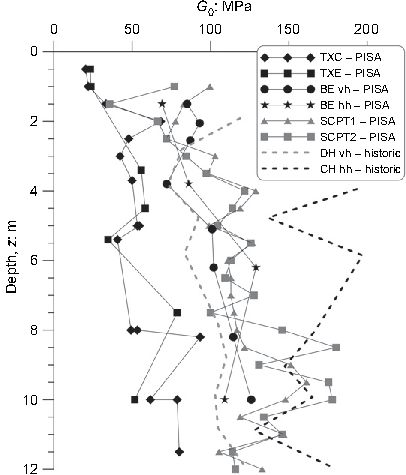
\includegraphics[width = 90mm]{Figures/figure-Cowden.pdf}
    \caption{Stiffness characteristics at Cowden. Source: \protect\cite{zdravkovic2020}}
    \label{fig: Cowden_cpt}
\end{figure}

To address these challenges in real time, digital twin (DT) has gained popularity in handling abundant data and predict the pile's response in a more organized and accurate manner \citep{wang2021}. DT makes full use of data such as physical models, sensor updates and operating history, and integrates simulation processes to real-time reproduce the dynamics of a physical system in the virtual space. More importantly, the DT model cannot only describe the current state of the physical entity, but also predict the future state. However, state-of-the-art digital twins are still relying on considerable expertise and deployment resources \citep{kapteyn2021}, leading to an only one-off implementation and remaining limitation on providing adaptive digital models on unique offshore piles. Thus, unified and scalable models should be developed and incorporated into digital twin to enable a intelligent decision making. Details about the need for unified and scalable digital twin for piles are outlined next.








\section{Urgent need for a unified and scalable digital twins for piles}
The demand for efficiency, reliability, and safety continues to grow in offshore wind foundation constructions. Computational models are an invaluable tool
 for understanding complex pile behaviors for new designs, operating conditions and control strategies. This reduces the need for costly experiments or field tests. However, insights gained from a computational model are contingent on the model being an accurate reflection of the underlying soil parameters. Moreover, real-world pile foundations are constantly changing and evolving throughout their lifecycle. Using a single static computational model that ignores these differences fundamentally limits the specificity,
 and thus the accuracy, of the model and any insights gained through its use.

 While the value proposition of digital twin has become widely appreciated in geotechnical engineering, the pile design process remains in a custom production phase. Current digital twin for offshore piles are still bespoken, relying on highly specialized implementations and thus requiring considerable resources and expertise to deploy and maintain. Therefore, it is necessary to move toward digital twins at scale by developing a rigorous and unified mathematical foundation. Based on a robust computational approach and  probabilistic graphical model \citep{kapteyn2021}, this unified mathematical foundation enables a promising application at scale in the offshore pile bearing response. 
 


\section{Objectives and outline}

The underlying objective of this thesis is to develop a robust and scalable digital twin model for offshore piles. This endeavor will leverage cutting-edge methodologies in surrogate modeling and uncertainty quantification, all geared towards facilitating extensive predictive digital twin capabilities. In particular, the specific goals of this thesis are:
\begin{itemize}[left=0pt]
    \item Develop a surrogate model suitable for offshore piles characterized by high input dimensions.
    
    \item Accelerate Bayesian inversion calculations for soil parameters to reduce the uncertainties, and providing real-time pile response predictions through adaptive enrichment of observed monitoring data.
    
    \item Develop a unifying mathematical foundation for predictive digital twins for offshore piles in the form of a probabilistic graphical model.
\end{itemize}